
\begin{table}[h!]
	\centering
	\caption{Divisão dos dados}
	\label{tab:divisao-dados}
\resizebox{\textwidth}{!}{
	\begin{tabular}{c c c c c c c c}
		\toprule
		\textbf{Abordagem} & \textbf{Característica} & \textbf{Tipo de Exemplo} & \textbf{Treino} & \textbf{Validação} & \textbf{Teste} & \textbf{Total} & \textbf{Proporção}\\
		\midrule
		\multirow{2}{*}{1} & \multirow{2}{*}{Dados desbalanceados} & Genuíno & 2.011 & 299 & 618 & 2.928 & $15\%$ \\
    &  & Forjado & 11.649 & 1.648 & 3.237 & 16.534 & $85\%$\\
     \midrule
    \multirow{2}{*}{2} & \multirow{2}{*}{Dados balanceados} & Genuíno & 2011 & 299 & 618 & & $50\%$  \\
    &  & Forjado & 2024 & 308 & 569 &  & $50\%$ \\
		 \midrule
		\multirow{2}{*}{3} & \multirow{2}{*}{Quasi-balanceados} & Genuíno & 2011 & 299 & 618  &  & \\
		 & & Forjado & 2024 & 308 & 569 & &\\
		\bottomrule
	\end{tabular}}
\end{table}

\todo{Preencher a tabela com novos valores.}

\begin{figure}[h!]
  \centering
\caption{Visualização da divisão dos dados}
  \subfloat[Abordagem 1\label{subfig:approach1}]{%
    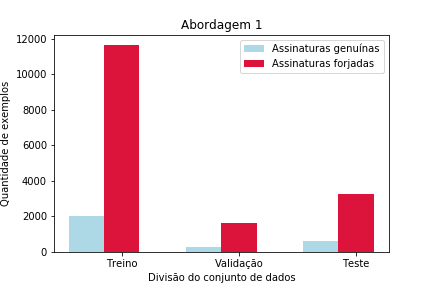
\includegraphics[width=0.7\textwidth]{imgs/approach1}
  }
  \hfill
  \subfloat[Abordagem 2\label{subfig:approach2}]{%
    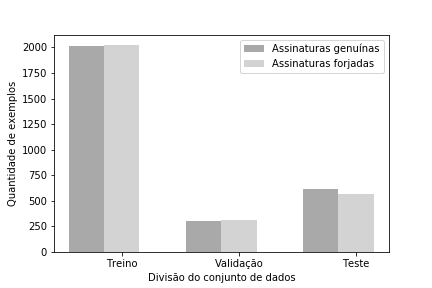
\includegraphics[width=0.7\textwidth]{imgs/approach2}
  }
  \label{fig:divisao-dados}
\end{figure}
